%!TEX root = ../thesis.tex

\section{実験装置}

  本研究で使用した実験装置を\figref{Fig:RobotGuidance_experiment_device}に示す.ハードウェアは,T-frogプロジェクトのi-Cart\ mini\cite{t-flog}をベースとしたロボットである,ORNE-box\cite{orne-box1}\cite{orne-box2}を使用する.このロボットは,拡張性に優れており,センサの取り付け位置を自由に変更できる.そのため,カメラを上部のハンドル部分に,2DLiDARを下部の足元付近に設置した.PCの仕様を\tabref{tab:Laptop computer specifications}に示す.また,ソフトウェアはROSを使用して構築し,深層学習のフレームワークにはPyTorchを採用している.

  \begin{figure}[h]
    \centering
    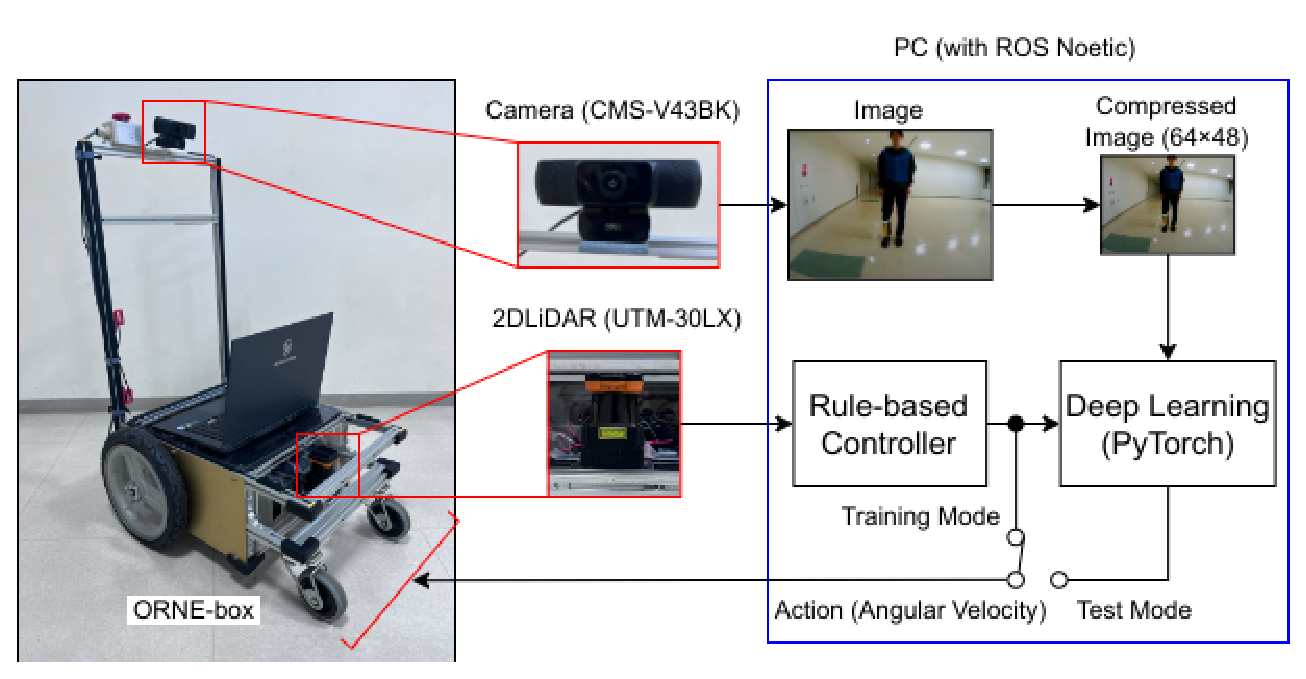
\includegraphics[keepaspectratio, scale=0.60] {images/eps/RobotGuidance_experiment_device}
    \captionsetup{justification=raggedright} % キャプションを左寄せに
    \caption{The developed system}
    \label{Fig:RobotGuidance_experiment_device}
  \end{figure}

  \begin{table}[h]
    \caption{Laptop computer specifications}
    \label{tab:Laptop computer specifications}
    \centering
    \begin{tabular}{cc}
    \hline
    Processor & Specification  \\
    \hline
    \hline
    OS   & Ubuntu 20.04 LTS                        \\ 
    ROS  & Noetic                                  \\ 
    CPU  & intel Core i7-10700F(4.8GHz/8コア/16スレッド) \\ 
    GPU  & RTX 2070 Max-Q                          \\ 
    DRAM & 32GB DDR4(3200/8GB × 4)                 \\ 
    \hline
    \end{tabular}
    \end{table}

\newpage
